\cleardoublepage
\chapter{Introduction}

\begin{chapterintro}

This chapters provides an introduction to the problem which will be approached in this project. It provides an overview of the benefits of mash-ups and linked data technologies. Furthermore, a deeper description of the project and its environment is also given.

\end{chapterintro}

\cleardoublepage
\section{Context}

The convergence of Telecom, IT and content services drives new emerging service markets based on an open Internet of Services. mash-ups have gained big success in the so-called Web 2.0. The success of the Web 2.0 services has encouraged Telcos to expose their services as Telco mash-ups, in order to provide third parties with facilities to build their business. Moreover, the exposure of network infrastructure as services is facilitating the entry of new API-driven telco agents that bring traditional telco services (telephony, messaging, IP location, etc.) to the Web.

Yet, the technologies underlying each of the different mash-up types are heterogeneous, which makes integration challenging. Also, mash-ups do not offer a universal composition model either, since mash-up development is not vendor independent. A mash-up developed within a specific technology has to be re-coded in order to be deployed in another engine.

This master thesis is developed as part of OMELETTE~\cite{chudnovskyy2012end} project which in turn is part of a FP7\footnote{FP7-ICT-2009-5} project that aims at researching on the development, management, governance, execution and conception of converged services with a specific focus on the Telco domain. OMELETTE will create a sound model of mash-ups that follows the REST architectural style (also supported by standard widget technology), as well as a standard specification of a mash-up-containing platform that may guarantee portability and interoperability among different vendors and versions. These concepts will be based on a solid theoretical model of mash-up foundations and the specific requirements gained from the telco domain. OMELETTE will foster as well the reuse of existing components and mash-ups, thanks to its automated service discovery functionalities. Project OMELETTE aims at developing an open platform for building convergent mash-ups for the telco domain to be used within several industry-driven use cases. 

\section{Master thesis description}

OMELETTE project provides end users an environment for developing and running widgets and mash-ups.  Users can create mash-ups with a mash-up editor and then run these mash-ups in the Live OMELETTE Environment as depicted in figure \ref{fig:generalpicture}.

The Live OMELETTE Environment interacts with the Service mash-up Environment (for direct deployment of new mash-ups), with the web, and with the OMELETTE Information Store (semantic storage of existing widgets and services).

For this master thesis \textbf{we are going to focus on how to discover and manage widgets and services} to develop new mash-ups (OMELETTE Information Store). We will integrate discovering techniques with the OMELETTE mash-up register (OMR) which is already developed and deployed.

\begin{figure}[ht]
	\centering
	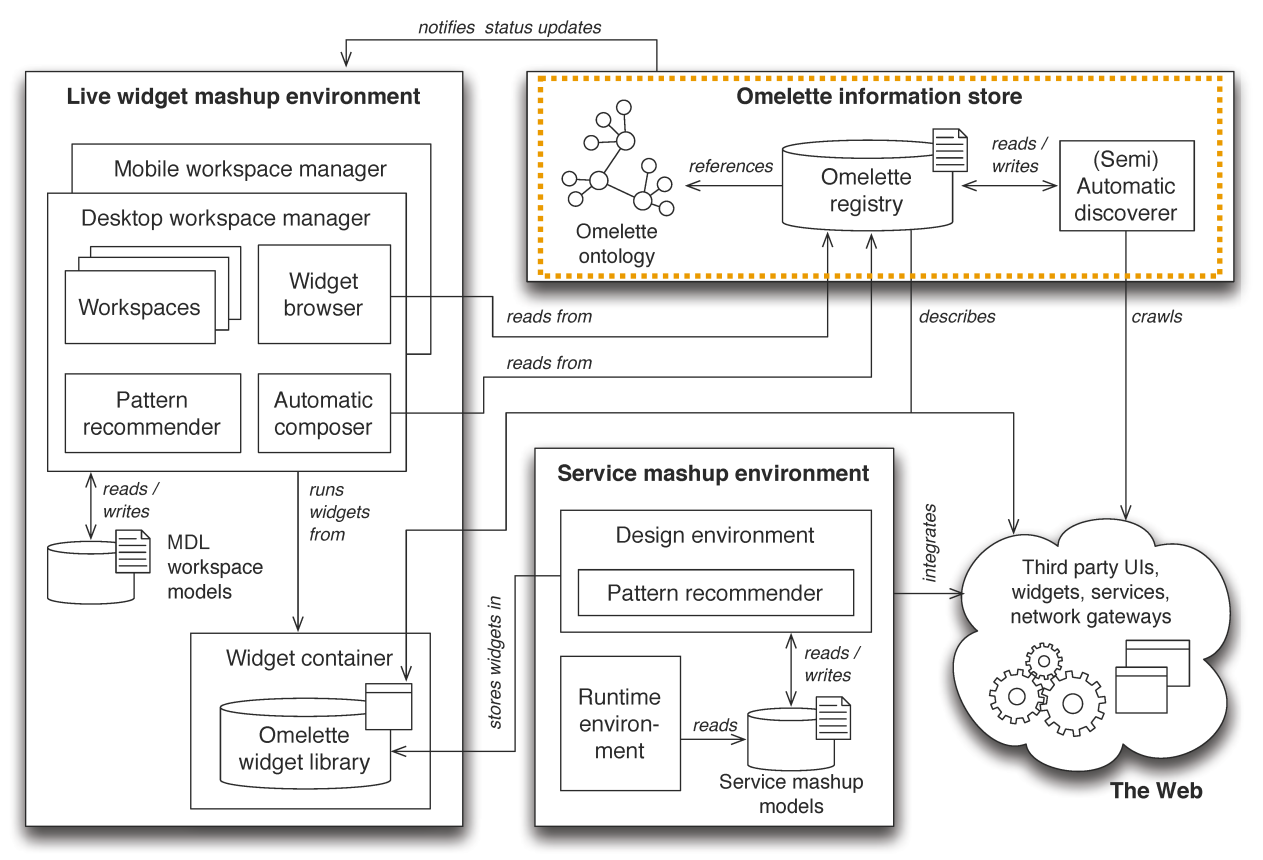
\includegraphics[width=400pt]{graphics/omelettegeneral.png}
	\caption{Omelette general picture}
	\label{fig:generalpicture}
\end{figure}

Inside the OMELETTE information store we distinguish the following modules:

\begin{description}

\item[OMELETTE mash-up Registry]  is the element that registers components for their usage by the rest of elements in the OMELETTE platform. A component can be a mash-up, a service, or a widget. Component descriptions and accompanying binary content will be stored in the OMR so that other elements from the OMELETTE architecture can query the OMR for them and use them. To describe components, a unified RDF component model has been defined. This unified component model provides a unified way to query components and identify, e.g., appropriate widgets for composition, interesting new services to be used when creating a widget, or relevant mash-ups of a particular domain.

\item[Automatic Discoverer] is the system responsible for populating the OMR with up-to-date components. In the current Web plenty of services and widgets are released every day, and developers need to be aware of these services in order to build state-of-the-art mash-ups. To achieve this, a module that crawls service and widget repositories registries these components into the OMR. This automatic discoverer produces semantic descriptions of the components found in the Web out of the unstructured HTML documents they are contained into.

\item[OMR admin interface] will allow to organize the components fetched by the automatic discoverer. Some of the components inserted into the OMR might be undesirable, and the administrator user within the admin interface will be responsible filter them.

\item[Web developer interface] will be used by final developer users allowing them to query by needs and recommending other services by using semantic search technologies.

\end{description}

\section{Master thesis goals}
\label{sec:masterthesisgoals}


The main purpose of this master thesis is to have a \textbf{repository} of widgets and services to build new mash-ups. First we need to \textbf{feed the repository} and we have to do it automatically using discovery techniques. The content fetched from the internet must be \textbf{structured} before it is inserted into the repository and therefore the repository has to be able to store the data with the same structure, this is done using \textbf{semantic repositories}.

All the information stored in the repository has to be \textbf{managed} manually by an administrator. This is the main goal of this master thesis, create an administration interface that permits an administrator user chose which widgets and services automatically fetched and stored are useful. The administrator interface will provide several tools to the administrator user and will use \textbf{ranking} algorithms to help him decide which ones are usefull.

Finally, there is a web interface for final users that will allow them find services and services using semantic search technologies.


\section{Structure of this Master Thesis}

In this section we will provide a brief overview of all the chapters of this Master Thesis. It
has been structured as follows:

\textit{Chapter 1} provides an introduction to the problem which will be approached in this project. It provides an overview of the benefits of mash-ups and linked data technologies. Furthermore, a deeper description of the project and its environment is also given.

\textit{Chapter 2} contains an overview of the existing technologies on which the development of the project will rely.

\textit{Chapter 3} describes one of the most important stages in software development: the requirement analysis using different scenarios. For this, a detailed analysis of the possible use cases is made using the Unified Modeling Language (UML). This language allows us to specify, build and document a system using graphic language.
The result of this evaluation will be a complete specification of the requirements, which will be matched by each module in the design stage. This helps us also to focus on key aspects and take apart other less important functionalities that could be implemented in future works.

\textit{Chapter 4} describes the architecture of the system, dividing it into 3 groups and differencing front-end and back-end modules.

\textit{Chapter 5} describes a selected use case. It is going to be explained the running of all the tools involved and its purpose. It is based on how to crawl the web to find new mash-ups, then feed the repository, do the validation and rejections of the mash-ups, and finally the developer will be able to use the discovered services.

\textit{Chapter 6} sums up the findings and conclusions found throughout the document and gives a hint about future development to continue the work done for this master thesis.

Finally, the appendix provide useful related information, especially covering the installation and configuration of the tools used in this thesis.